\subsection{Data fields}
\label{subsec:library_of_transformations:type_level_transformations:data_fields}

\begin{figure}
    \centering
    \begin{subfigure}{0.45\textwidth}
        \centering
        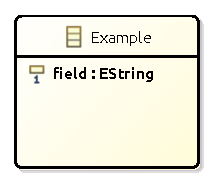
\includegraphics{images/05_library_of_transformations/02_type_level_transformations/06_data_fields/data_field.pdf}
        \caption{$Tm_{DataField}$ for a $\type{string}$ with $name = \type{field}$}
        \label{fig:library_of_transformations:type_level_transformations:data_fields:visualisation:ecore}
    \end{subfigure}
    \begin{subfigure}{0.45\textwidth}
        \centering
        % To use this figure in your LaTeX document
% import the package groove/resources/groove2tikz.sty
%
\begin{tikzpicture}[scale=\tikzscale,name prefix=test-]
\node[type_node] (n0) at (0.955, -0.775) {\ml{\textbf{Example}\\field: \textbf{string}}};

\end{tikzpicture}

        \caption{$TG_{DataField}$ for a $\type{string}$ with $name = \type{field}$}
        \label{fig:library_of_transformations:type_level_transformations:data_fields:visualisation:groove}
    \end{subfigure}
    \caption{Visualisation of the transformation of a field typed by a data type}
    \label{fig:library_of_transformations:type_level_transformations:data_fields:visualisation}
\end{figure}

All transformations discussed so far have focused on introducing different kind of types. In the following transformations, these types will be enriched with fields. In this transformation specifically, a field typed by a data type will be introduced.

\begin{defin}[Type model $Tm_{DataField}$]
\label{defin:library_of_transformations:type_level_transformations:data_fields:tmod_data_field}
Let $Tm_{DataField}$ be the type model containing a regular class with identifier $classtype$. Then $Tm_{DataField}$ defines a field named $name$ with type $fieldtype$, in which $fieldtype$ is either $\type{boolean}$, $\type{integer}$, $\type{real}$ or $\type{string}$. $Tm_{DataField}$ is defined as:
\begin{align*}
Class =\ &\{classtype\} \\
Enum =\ &\{\} \\
UserDataType =\ &\{\} \\
Field =\ &\{(classtype, name)\} \\
\mathrm{FieldSig} =\ &\begin{cases}
    (f, (fieldtype, 1..1)) &\mathrm{if}\ f \in Field_{Tm_{DataField}}
\end{cases} \\
EnumValue =\ &\{\} \\
Inh =\ &\{\} \\
Prop =\ &\{\} \\
Constant =\ &\{\} \\
\mathrm{ConstType} =\ &\{\}
\end{align*}
\isabellelref{tmod_data_field}{Ecore-GROOVE-Mapping-Library.DataField}
\end{defin}

\begin{thm}[Correctness of $Tm_{DataField}$]
\label{defin:library_of_transformations:type_level_transformations:data_fields:tmod_data_field_correct}
$Tm_{DataField}$ (\cref{defin:library_of_transformations:type_level_transformations:data_fields:tmod_data_field}) is a consistent type model in the sense of \cref{defin:formalisations:ecore_formalisation:type_models:type_model_consistency}.
\isabellelref{tmod_data_field_correct}{Ecore-GROOVE-Mapping-Library.DataField}
\end{thm}

A visual representation of $Tm_{DataField}$ with field name $\type{field}$ on class $.\type{Example}$ can be seen in \cref{fig:library_of_transformations:type_level_transformations:data_fields:visualisation:ecore}. In this example, the $\type{string}$ type is chosen for the fieldtype, but any data type would have worked. The correctness proof of $Tm_{DataField}$ is more involved, it is not included here for conciseness. It can be found within the validated Isabelle proofs.

In order to make composing transformation functions possible, $Tm_{DataField}$ should be compatible with the type model it is combined with.

\begin{thm}[Correctness of $\mathrm{combine}(Tm, Tm_{DataField})$]
\label{defin:library_of_transformations:type_level_transformations:data_fields:tmod_data_field_combine_correct}
Assume a type model $Tm$ that is consistent in the sense of \cref{defin:formalisations:ecore_formalisation:type_models:type_model_consistency}. Then $Tm$ is compatible with $Tm_{DataField}$ (in the sense of \cref{defin:transformation_framework:type_models_and_type_graphs:combining_type_models:compatibility}) if:
\begin{itemize}
    \item The class type on which the field is defined, $classtype$, is already an existing class in $Tm$;
    \item The field named $name$ is not already a field on $classtype$ in $Tm$.
\end{itemize}
\isabellelref{tmod_data_field_combine_correct}{Ecore-GROOVE-Mapping-Library.DataField}
\end{thm}

\begin{proof}
Use \cref{defin:transformation_framework:type_models_and_type_graphs:combining_type_models:tmod_combine_merge_correct}. It is possible to show that all assumptions hold. Now we have shown that $\mathrm{combine}(Tm, Tm_{DataField})$ is consistent in the sense of \cref{defin:formalisations:ecore_formalisation:type_models:type_model_consistency}.
\end{proof}

The definitions and theorems for defining a data field within Ecore are now complete. 

\subsubsection{Encoding as edge type}

The most obvious encoding for an field in GROOVE would be using an edge type. The field is transformed into an edge type between an existing node type and the corresponding field type. The encoding corresponding to $Tm_{DataField}$ can then be represented as $TG_{DataField}$, defined in the following definition:

\begin{defin}[Type graph $TG_{DataField}$]
\label{defin:library_of_transformations:type_level_transformations:data_fields:tg_data_field_as_edge_type}
Let $TG_{DataField}$ be the type graph containing a node type which encodes the class type $classtype$. Furthermore, define an edge type from $classtype$ named $name$. This edge type targets a node of $fieldtype$. $TG_{DataField}$ is defined as:
\begin{align*}
NT =\ &\{\mathrm{ns\_\!to\_\!list}(classtype), fieldtype\} \\
ET =\ &\{(\mathrm{ns\_\!to\_\!list}(classtype), \langle name \rangle, fieldtype)\} \\
\!\!\sqsubseteq\ =\ &\{( \mathrm{ns\_\!to\_\!list}(classtype), \mathrm{ns\_\!to\_\!list}(classtype) ), ( fieldtype, fieldtype )\} \\
abs =\ &\{\} \\
\mathrm{mult}(e) =\ &\begin{cases}
    (0..\mstar, 1..1) &\mathrm{if}\ e \in \{(\mathrm{ns\_\!to\_\!list}(classtype), \langle name \rangle, fieldtype)\}
\end{cases} \\
contains =\ &\{\}
\end{align*}
\isabellelref{tg_data_field_as_edge_type}{Ecore-GROOVE-Mapping-Library.DataField}
\end{defin}

\begin{thm}[Correctness of $TG_{DataField}$]
\label{defin:library_of_transformations:type_level_transformations:data_fields:tg_data_field_as_edge_type_correct}
$TG_{DataField}$ (\cref{defin:library_of_transformations:type_level_transformations:data_fields:tg_data_field_as_edge_type}) is a valid type graph in the sense of \cref{defin:formalisations:groove_formalisation:type_graphs:type_graph_validity}.
\isabellelref{tg_data_field_as_edge_type_correct}{Ecore-GROOVE-Mapping-Library.DataField}
\end{thm}

A visual representation of $TG_{DataField}$ with edge name $\type{field}$ on node type $\type{Example}$ can be seen in \cref{fig:library_of_transformations:type_level_transformations:data_fields:visualisation:groove}. Like the previous example, a $\type{string}$ has been chosen to be consequent, but any primitive type could have been used. The correctness proof of $TG_{DataField}$ is more involved, it is not included here for conciseness. It can be found within the validated Isabelle proofs.

In order to make composing transformation functions possible, $TG_{DataField}$ should be compatible with the type graph it is combined with.

\begin{thm}[Correctness of $\mathrm{combine}(TG, TG_{DataField})$]
\label{defin:library_of_transformations:type_level_transformations:data_fields:tg_data_field_as_edge_type_combine_correct}
Assume a type graph $TG$ that is valid in the sense of \cref{defin:formalisations:groove_formalisation:type_graphs:type_graph_validity}. Then $TG$ is compatible with $TG_{DataField}$ (in the sense of \cref{defin:transformation_framework:type_models_and_type_graphs:combining_type_graphs:compatibility}) if:
\begin{itemize}
    \item The node type of the encoded class type in $TG_{DataField}$ is already an node type in $TG$;
    \item The node type of the encoded class type in $TG_{DataField}$ does not already have an edge type with the same name as the field in $TG$.
\end{itemize}
\isabellelref{tg_data_field_as_edge_type_combine_correct}{Ecore-GROOVE-Mapping-Library.DataField}
\end{thm}

\begin{proof}
Use \cref{defin:transformation_framework:type_models_and_type_graphs:combining_type_graphs:tg_combine_merge_correct}. It is possible to show that all assumptions hold. Now we have shown that $\mathrm{combine}(TG, TG_{DataField})$ is valid in the sense of \cref{defin:formalisations:groove_formalisation:type_graphs:type_graph_validity}.
\end{proof}

The next definitions define the transformation function from $Tm_{DataField}$ to $TG_{DataField}$:

\begin{defin}[Transformation function $f_{DataField}$]
\label{defin:library_of_transformations:type_level_transformations:data_fields:tmod_data_field_to_tg_data_field_as_edge_type}
The transformation function $f_{DataField}(Tm)$ is defined as:
\begin{align*}
NT =\ &\{\mathrm{ns\_\!to\_\!list}(c) \mid c \in Class_{Tm}\} \cup \{fieldtype\}\\
ET =\ &\{(\mathrm{ns\_\!to\_\!list}(c), \langle f \rangle, fieldtype) \mid (c, n) \in Field_{Tm} \} \\
\!\!\sqsubseteq\ =\ &\{( \mathrm{ns\_\!to\_\!list}(c), \mathrm{ns\_\!to\_\!list}(c) ) \mid c \in Class_{Tm} \} \cup \{( fieldtype, fieldtype ) \} \\
abs =\ &\{\} \\
\mathrm{mult} =\ &\begin{cases}
    (0..\mstar, 1..1) &\mathrm{if}\ e \in \{(\mathrm{ns\_\!to\_\!list}(c), \langle f \rangle, fieldtype) \mid (c, n) \in Field_{Tm} \}
\end{cases} \\
contains =\ &\{\}
\end{align*}
\isabellelref{tmod_data_field_to_tg_data_field_as_edge_type}{Ecore-GROOVE-Mapping-Library.DataField}
\end{defin}

\begin{thm}[Correctness of $f_{DataField}$]
\label{defin:library_of_transformations:type_level_transformations:data_fields:tmod_data_field_to_tg_data_field_as_edge_type_func}
$f_{DataField}(Tm)$ (\cref{defin:library_of_transformations:type_level_transformations:data_fields:tmod_data_field_to_tg_data_field_as_edge_type}) is a valid transformation function in the sense of \cref{defin:transformation_framework:type_models_and_type_graphs:combining_transformation_functions:transformation_function_type_model_type_graph} transforming $Tm_{DataField}$ into $TG_{DataField}$.
\isabellelref{tmod_data_field_to_tg_data_field_as_edge_type_func}{Ecore-GROOVE-Mapping-Library.DataField}
\end{thm}

The proof of the correctness of $f_{DataField}$ will not be included here. Instead, it can be found in the validated Isabelle theories.

Finally, to complete the transformation, the transformation function that transforms $TG_{DataField}$ into $Tm_{DataField}$ is defined:

\begin{defin}[Transformation function $f'_{DataField}$]
\label{defin:library_of_transformations:type_level_transformations:data_fields:tg_data_field_as_edge_type_to_tmod_data_field}
The transformation function $f'_{DataField}(TG)$ is defined as:
\begin{align*}
Class =\ &\{\mathrm{list\_\!to\_\!ns}(n) \mid n \in NT_{TG} \cap Lab_t \} \\
Enum =\ &\{\} \\
UserDataType =\ &\{\} \\
Field =\ &\{(\mathrm{list\_\!to\_\!ns}(\mathrm{src}(e)), l) \mid e \in ET_{TG} \land \langle l \rangle = \mathrm{lab}(e) \} \\
\mathrm{FieldSig} =\ &\begin{cases}
    (f, (fieldtype, 1..1)) &\mathrm{if}\ f \in \{(\mathrm{list\_\!to\_\!ns}(\mathrm{src}(e)), l) \mid e \in ET_{TG} \land \langle l \rangle = \mathrm{lab}(e) \} 
\end{cases} \\
EnumValue =\ &\{\} \\
Inh =\ &\{\} \\
Prop =\ &\{\} \\
Constant =\ &\{\} \\
\mathrm{ConstType} =\ &\{\}
\end{align*}
\isabellelref{tg_data_field_as_edge_type_to_tmod_data_field}{Ecore-GROOVE-Mapping-Library.DataField}
\end{defin}

\begin{thm}[Correctness of $f'_{DataField}$]
\label{defin:library_of_transformations:type_level_transformations:data_fields:tg_data_field_as_edge_type_to_tmod_data_field_func}
$f'_{DataField}(TG)$ (\cref{defin:library_of_transformations:type_level_transformations:data_fields:tg_data_field_as_edge_type_to_tmod_data_field}) is a valid transformation function in the sense of \cref{defin:transformation_framework:type_models_and_type_graphs:combining_transformation_functions:transformation_function_type_graph_type_model} transforming $TG_{DataField}$ into $Tm_{DataField}$.
\isabellelref{tg_data_field_as_edge_type_to_tmod_data_field_func}{Ecore-GROOVE-Mapping-Library.DataField}
\end{thm}

Once more, the correctness proof is not included here but can be found in the validated Isabelle proofs of this thesis.